
% Anexo
%--------------------------------------
\vspace*{45pt}
% Título do anexo B (\tituloanexoB) definido no ficheiro main
\section*{Anexo B - \tituloanexoB}

This appendix presents representative output screens produced by the web platform, including Gene Ontology prediction, 2D HP lattice visualization with step-by-step exploration, and interactive 3D structure retrieval.

\begin{figure}[!htbp]
\centering
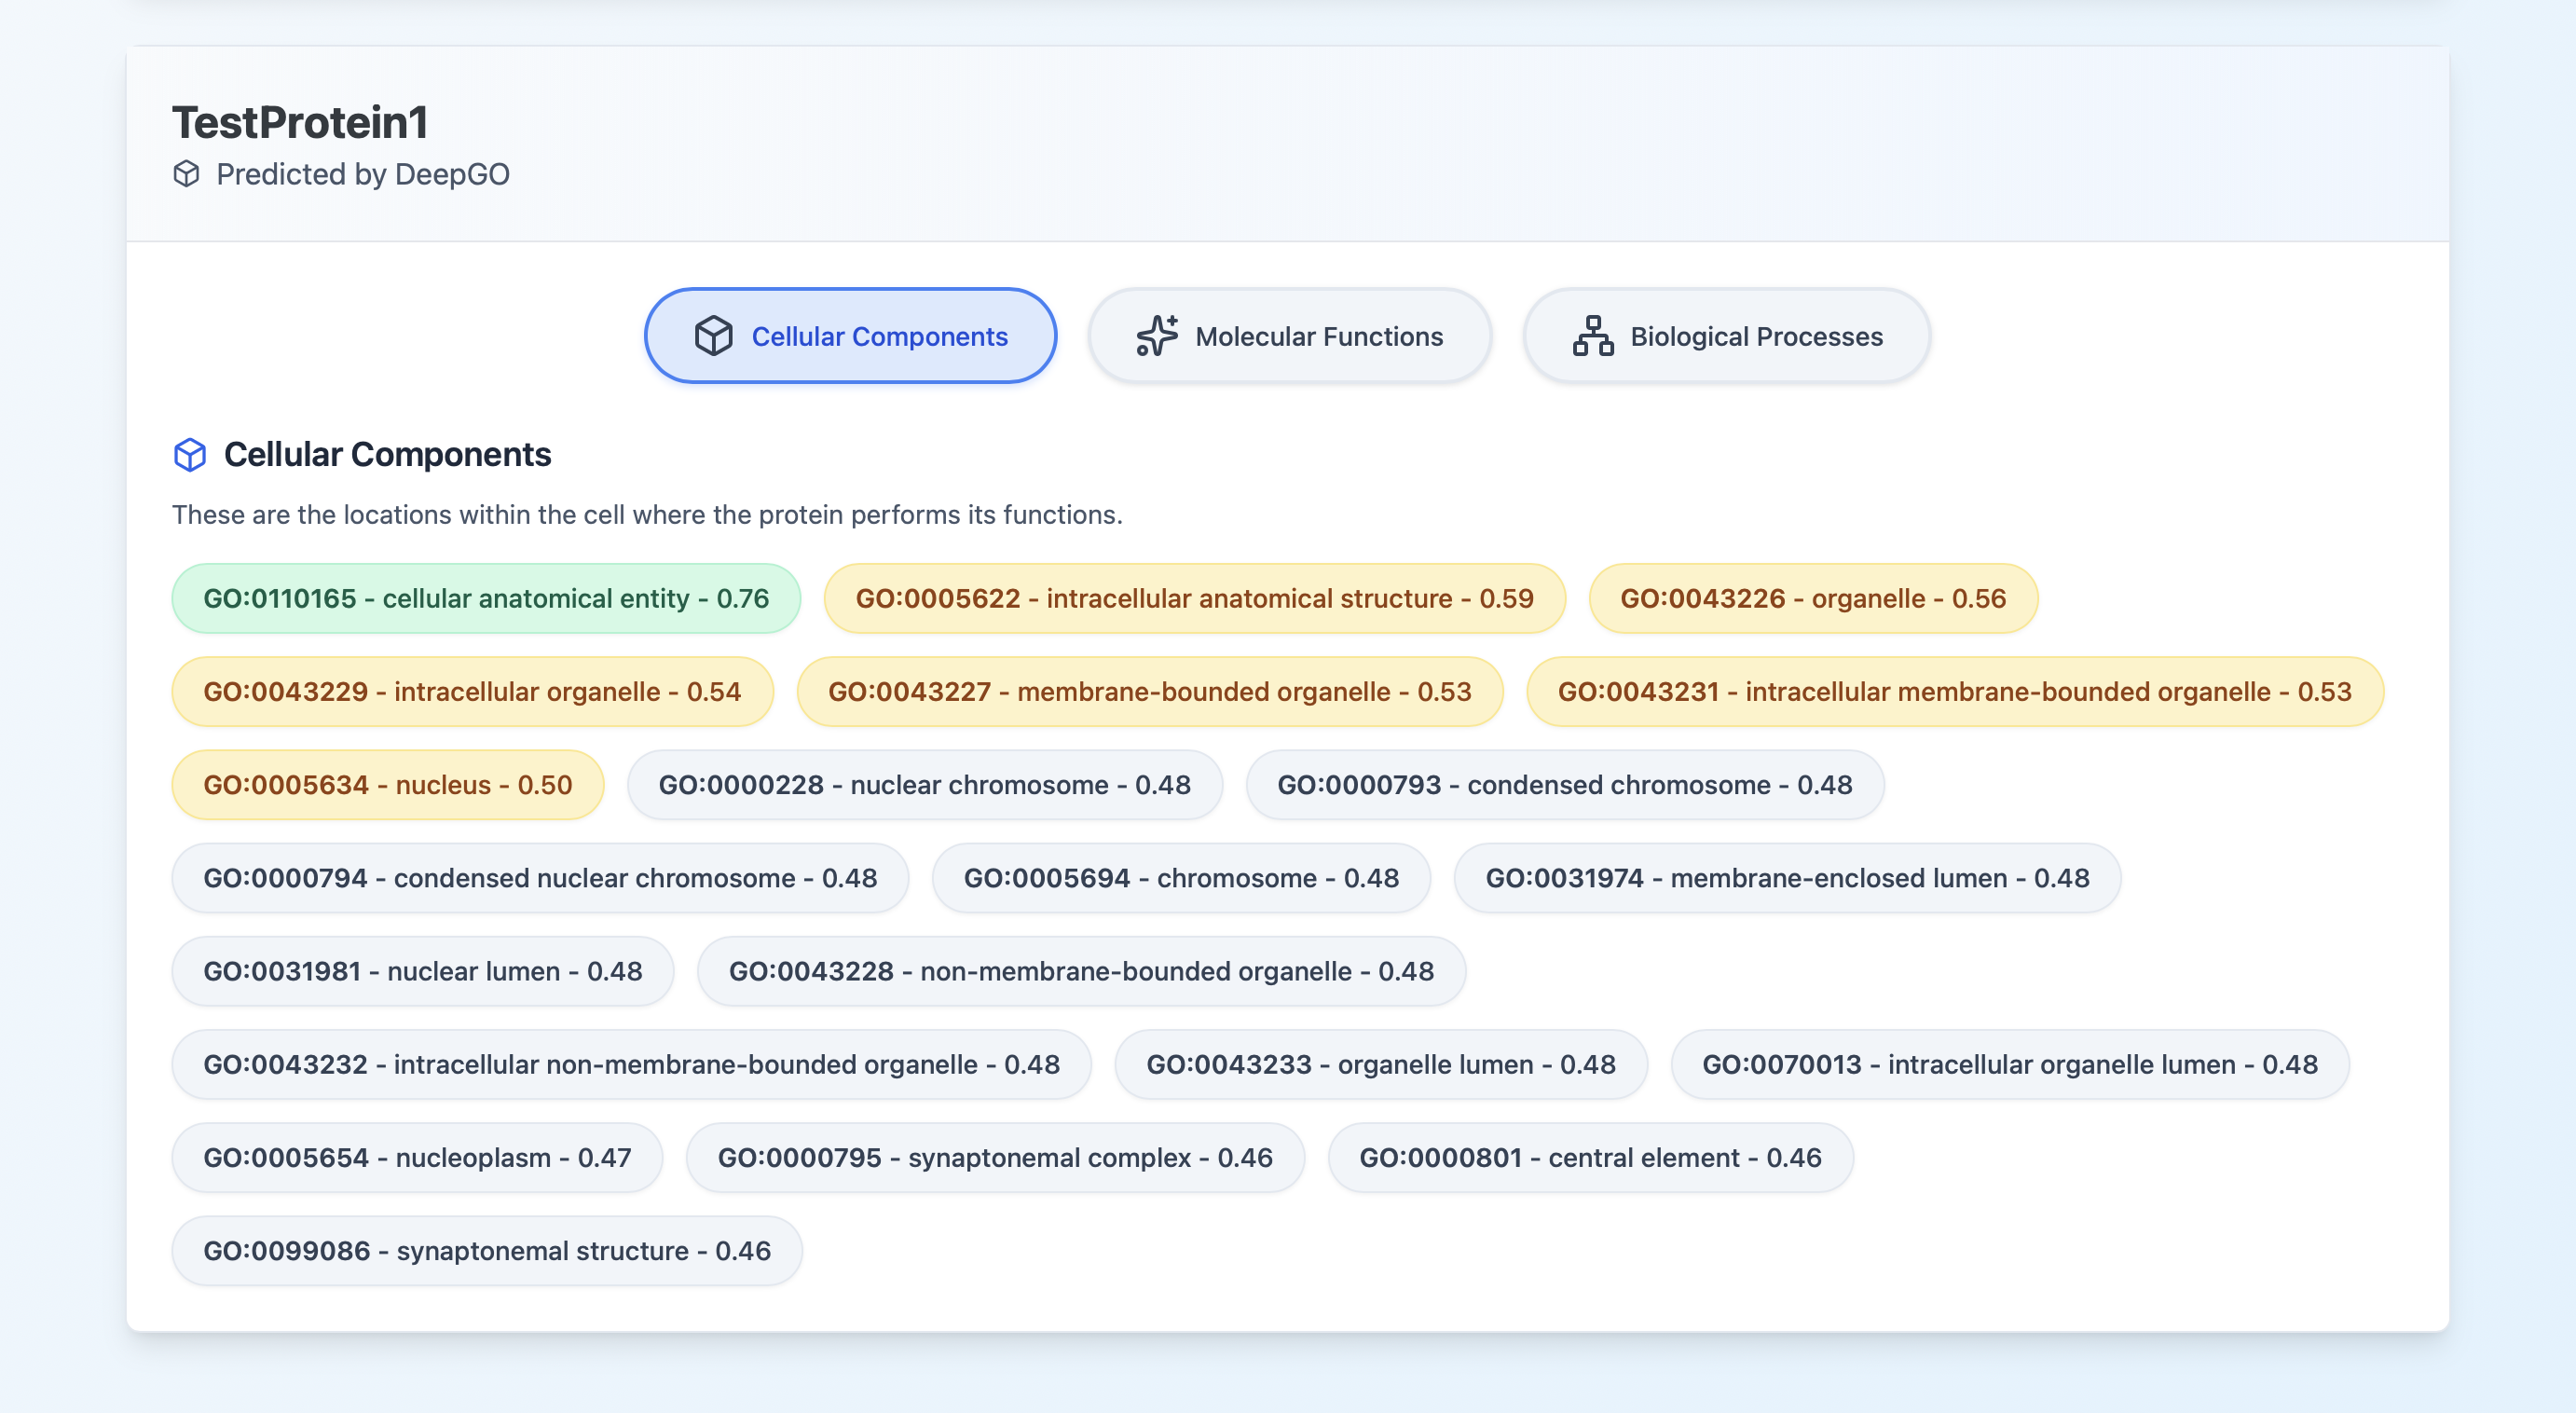
\includegraphics[width=\textwidth,height=0.76\textheight,keepaspectratio]{Figuras/goTermsResult.png}
\caption[GO prediction results screen]{GO prediction results screen. Predicted Gene Ontology terms are grouped by biological process, molecular function, and cellular component when returned by the external DeepGO service.}
\label{fig:appendix_go_results}
\end{figure}
\FloatBarrier

Figures~\ref{fig:appendix_2d_structure_step_initial}--\ref{fig:appendix_2d_structure_step_final} illustrate the step explorer added to the 2D structure visualization workflow. Instead of showing only the final conformation, the platform stores intermediate frames according to the user-defined interval and lets the user navigate the folding trajectory with previous, play, next, and slider controls. For the constructive DQN, each displayed step corresponds to one or more residues added during chain construction; for classical algorithms, each displayed step corresponds to a sampled optimization interval.

In the deployed web version, the number of DQN rollouts was scaled down due to the limited computational resources of the hosting environment.

\begin{figure}[!htbp]
\centering
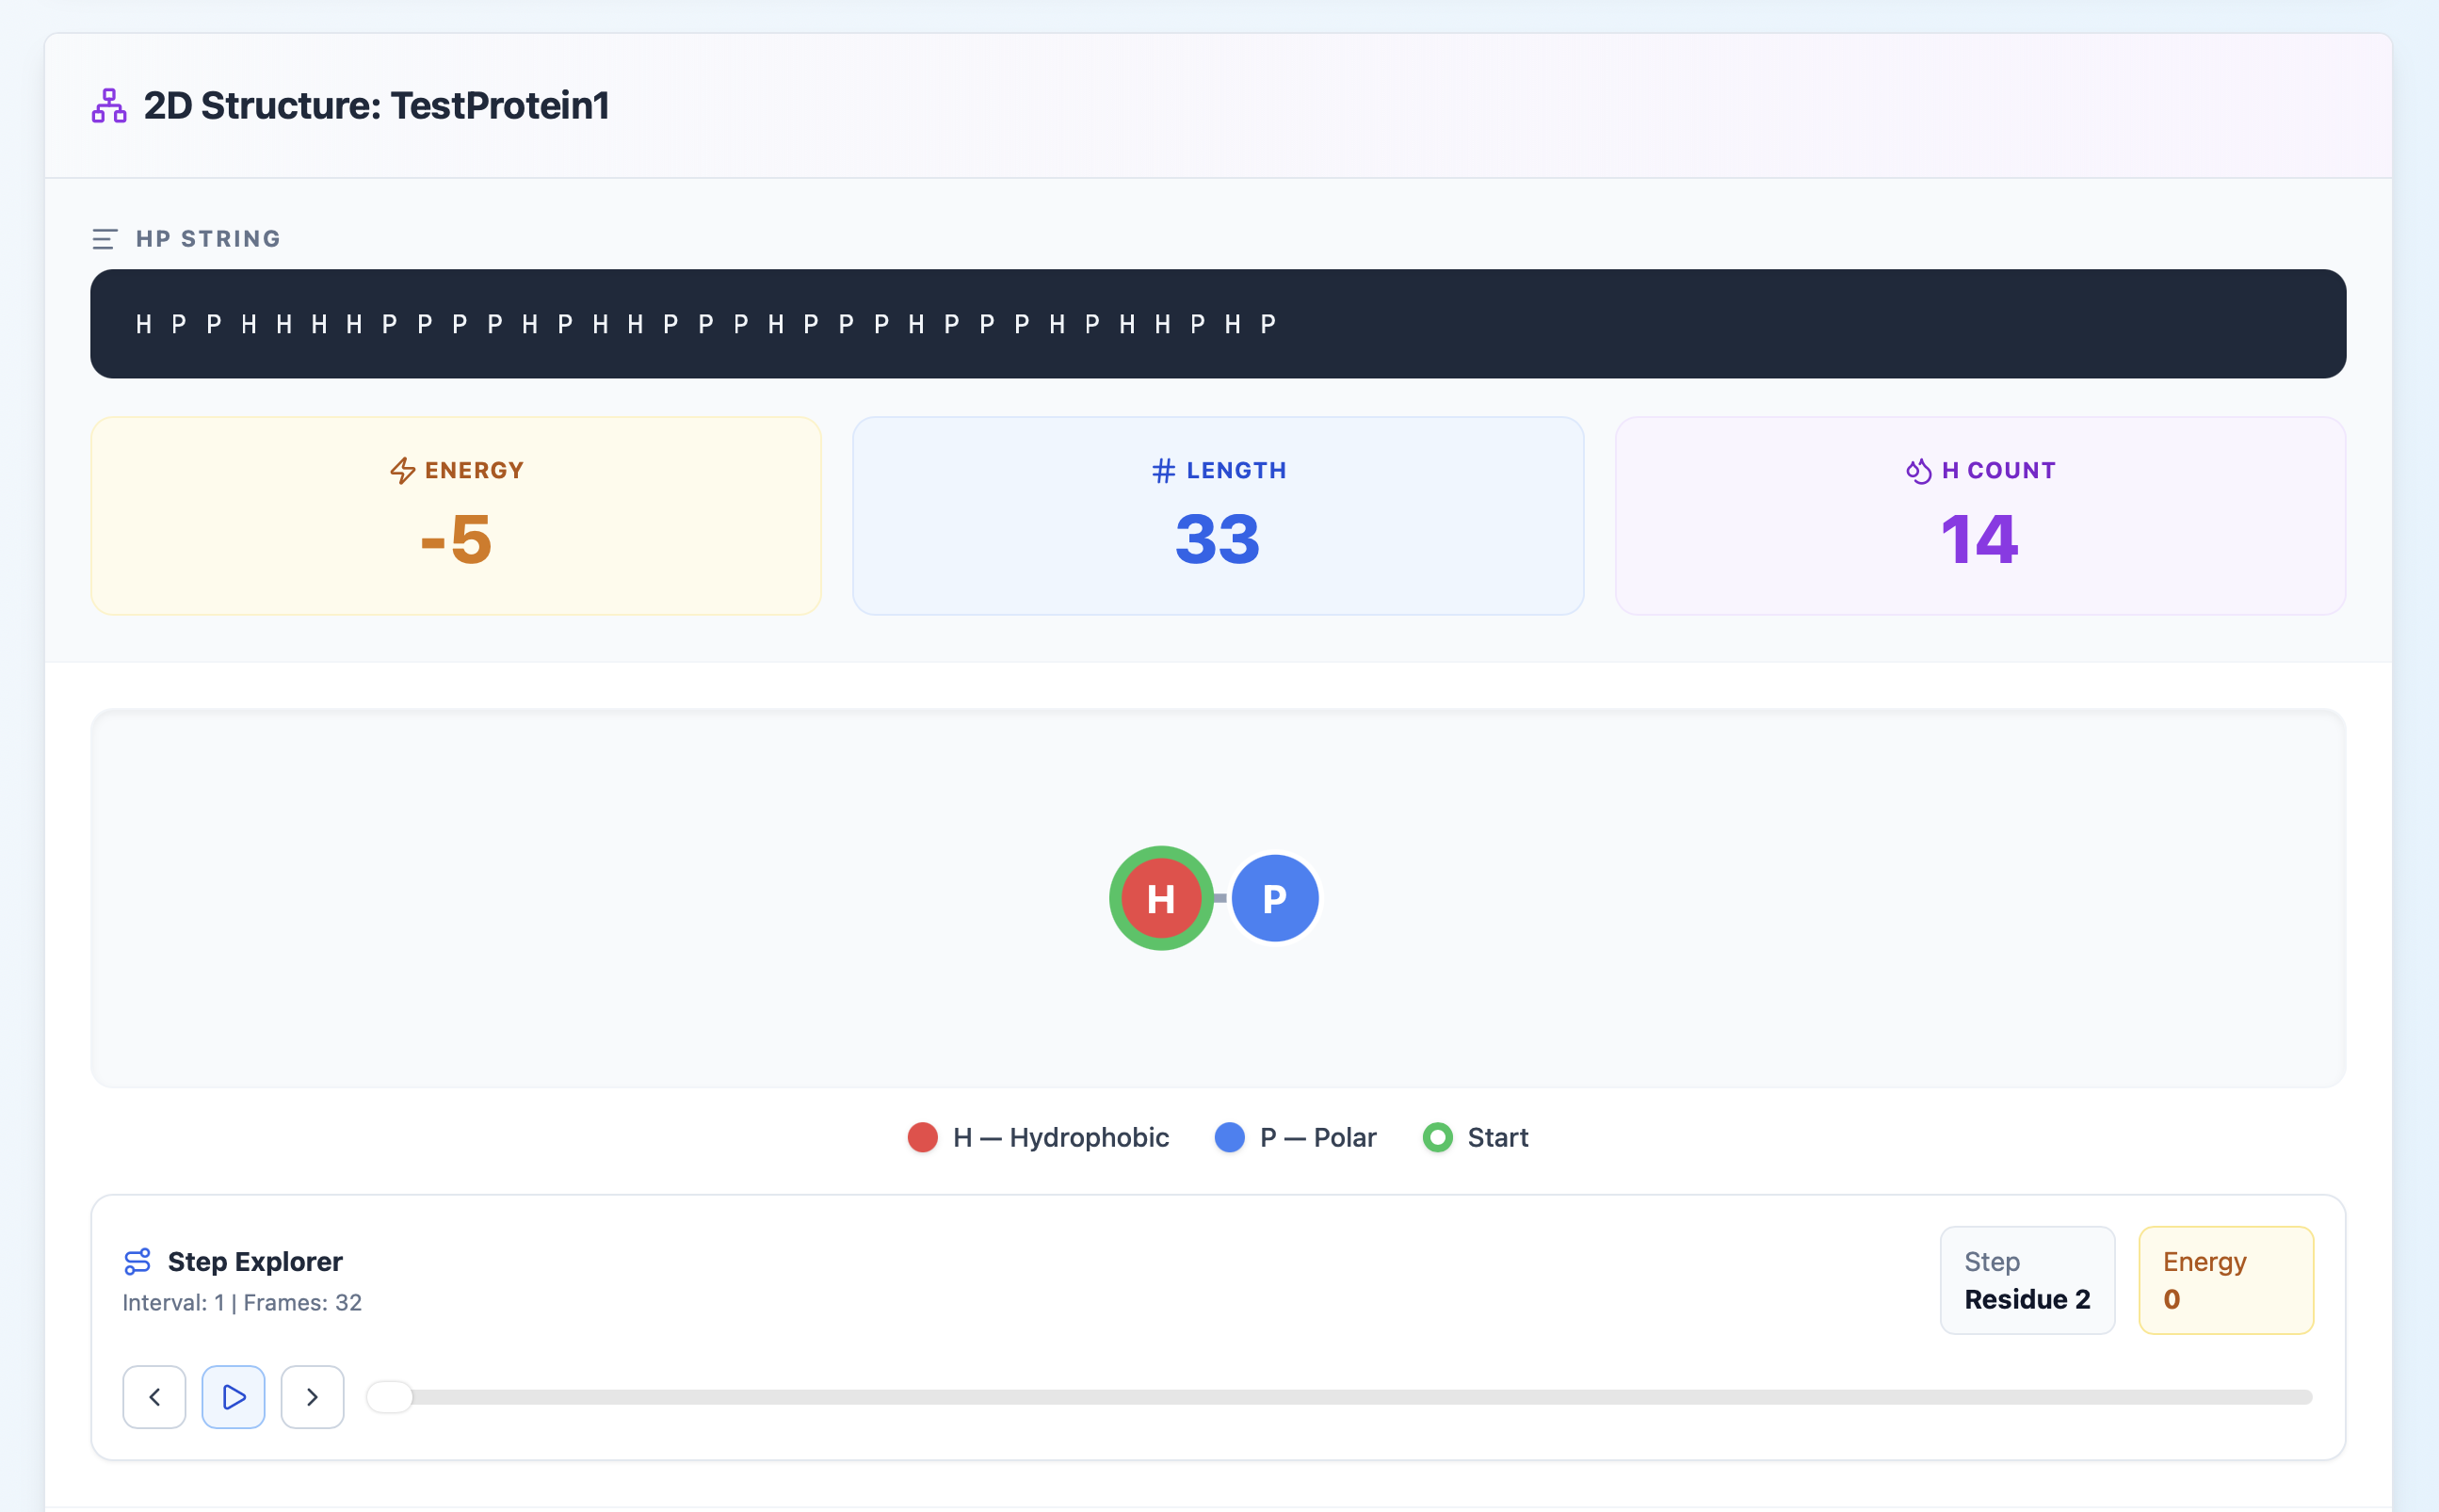
\includegraphics[width=\textwidth,height=0.70\textheight,keepaspectratio]{Figuras/2dStructure.png}
\caption[2D HP step explorer: initial frame]{Initial 2D HP step-explorer frame. The protein construction starts from the first residues, with the current step, energy, frame count, and playback controls displayed below the SVG lattice.}
\label{fig:appendix_2d_structure_step_initial}
\end{figure}
\FloatBarrier

\begin{figure}[!htbp]
\centering
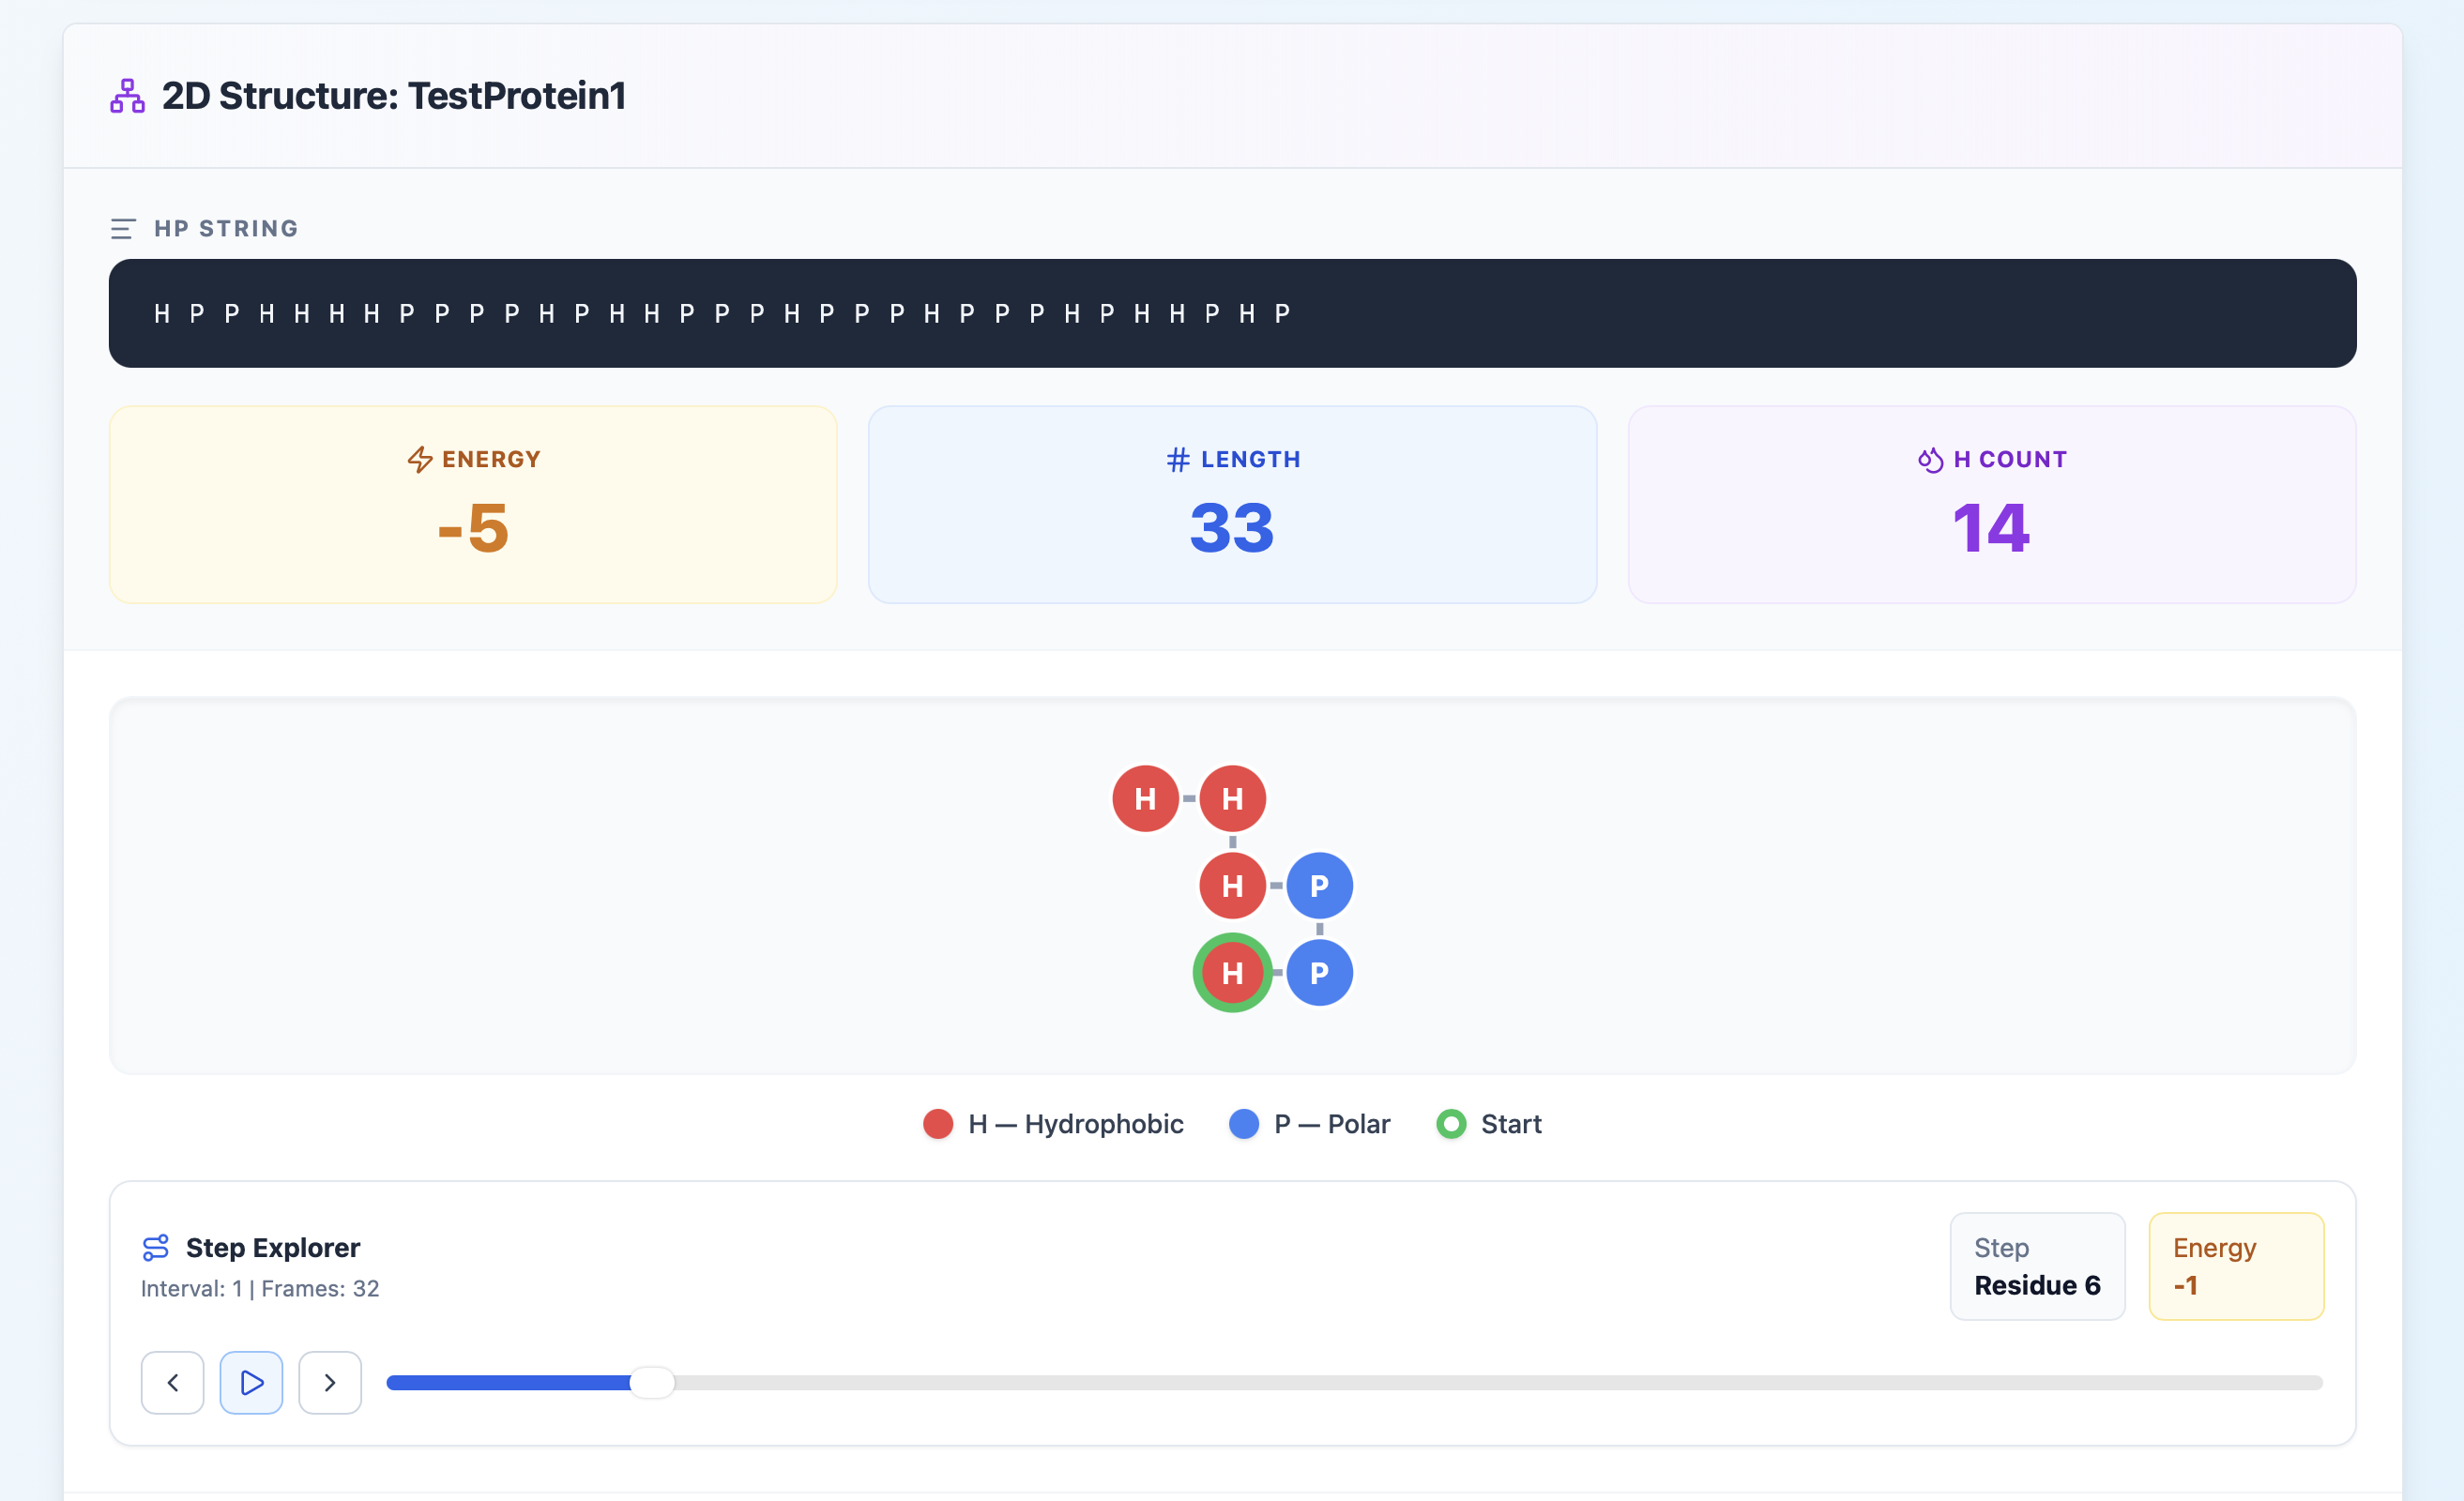
\includegraphics[width=\textwidth,height=0.70\textheight,keepaspectratio]{Figuras/2dStructure2.png}
\caption[2D HP step explorer: early folding frame]{Early folding frame in the 2D HP step explorer. The interface shows how the partial chain grows while preserving the same energy, sequence, and navigation context.}
\label{fig:appendix_2d_structure_step_early}
\end{figure}
\FloatBarrier

\begin{figure}[!htbp]
\centering
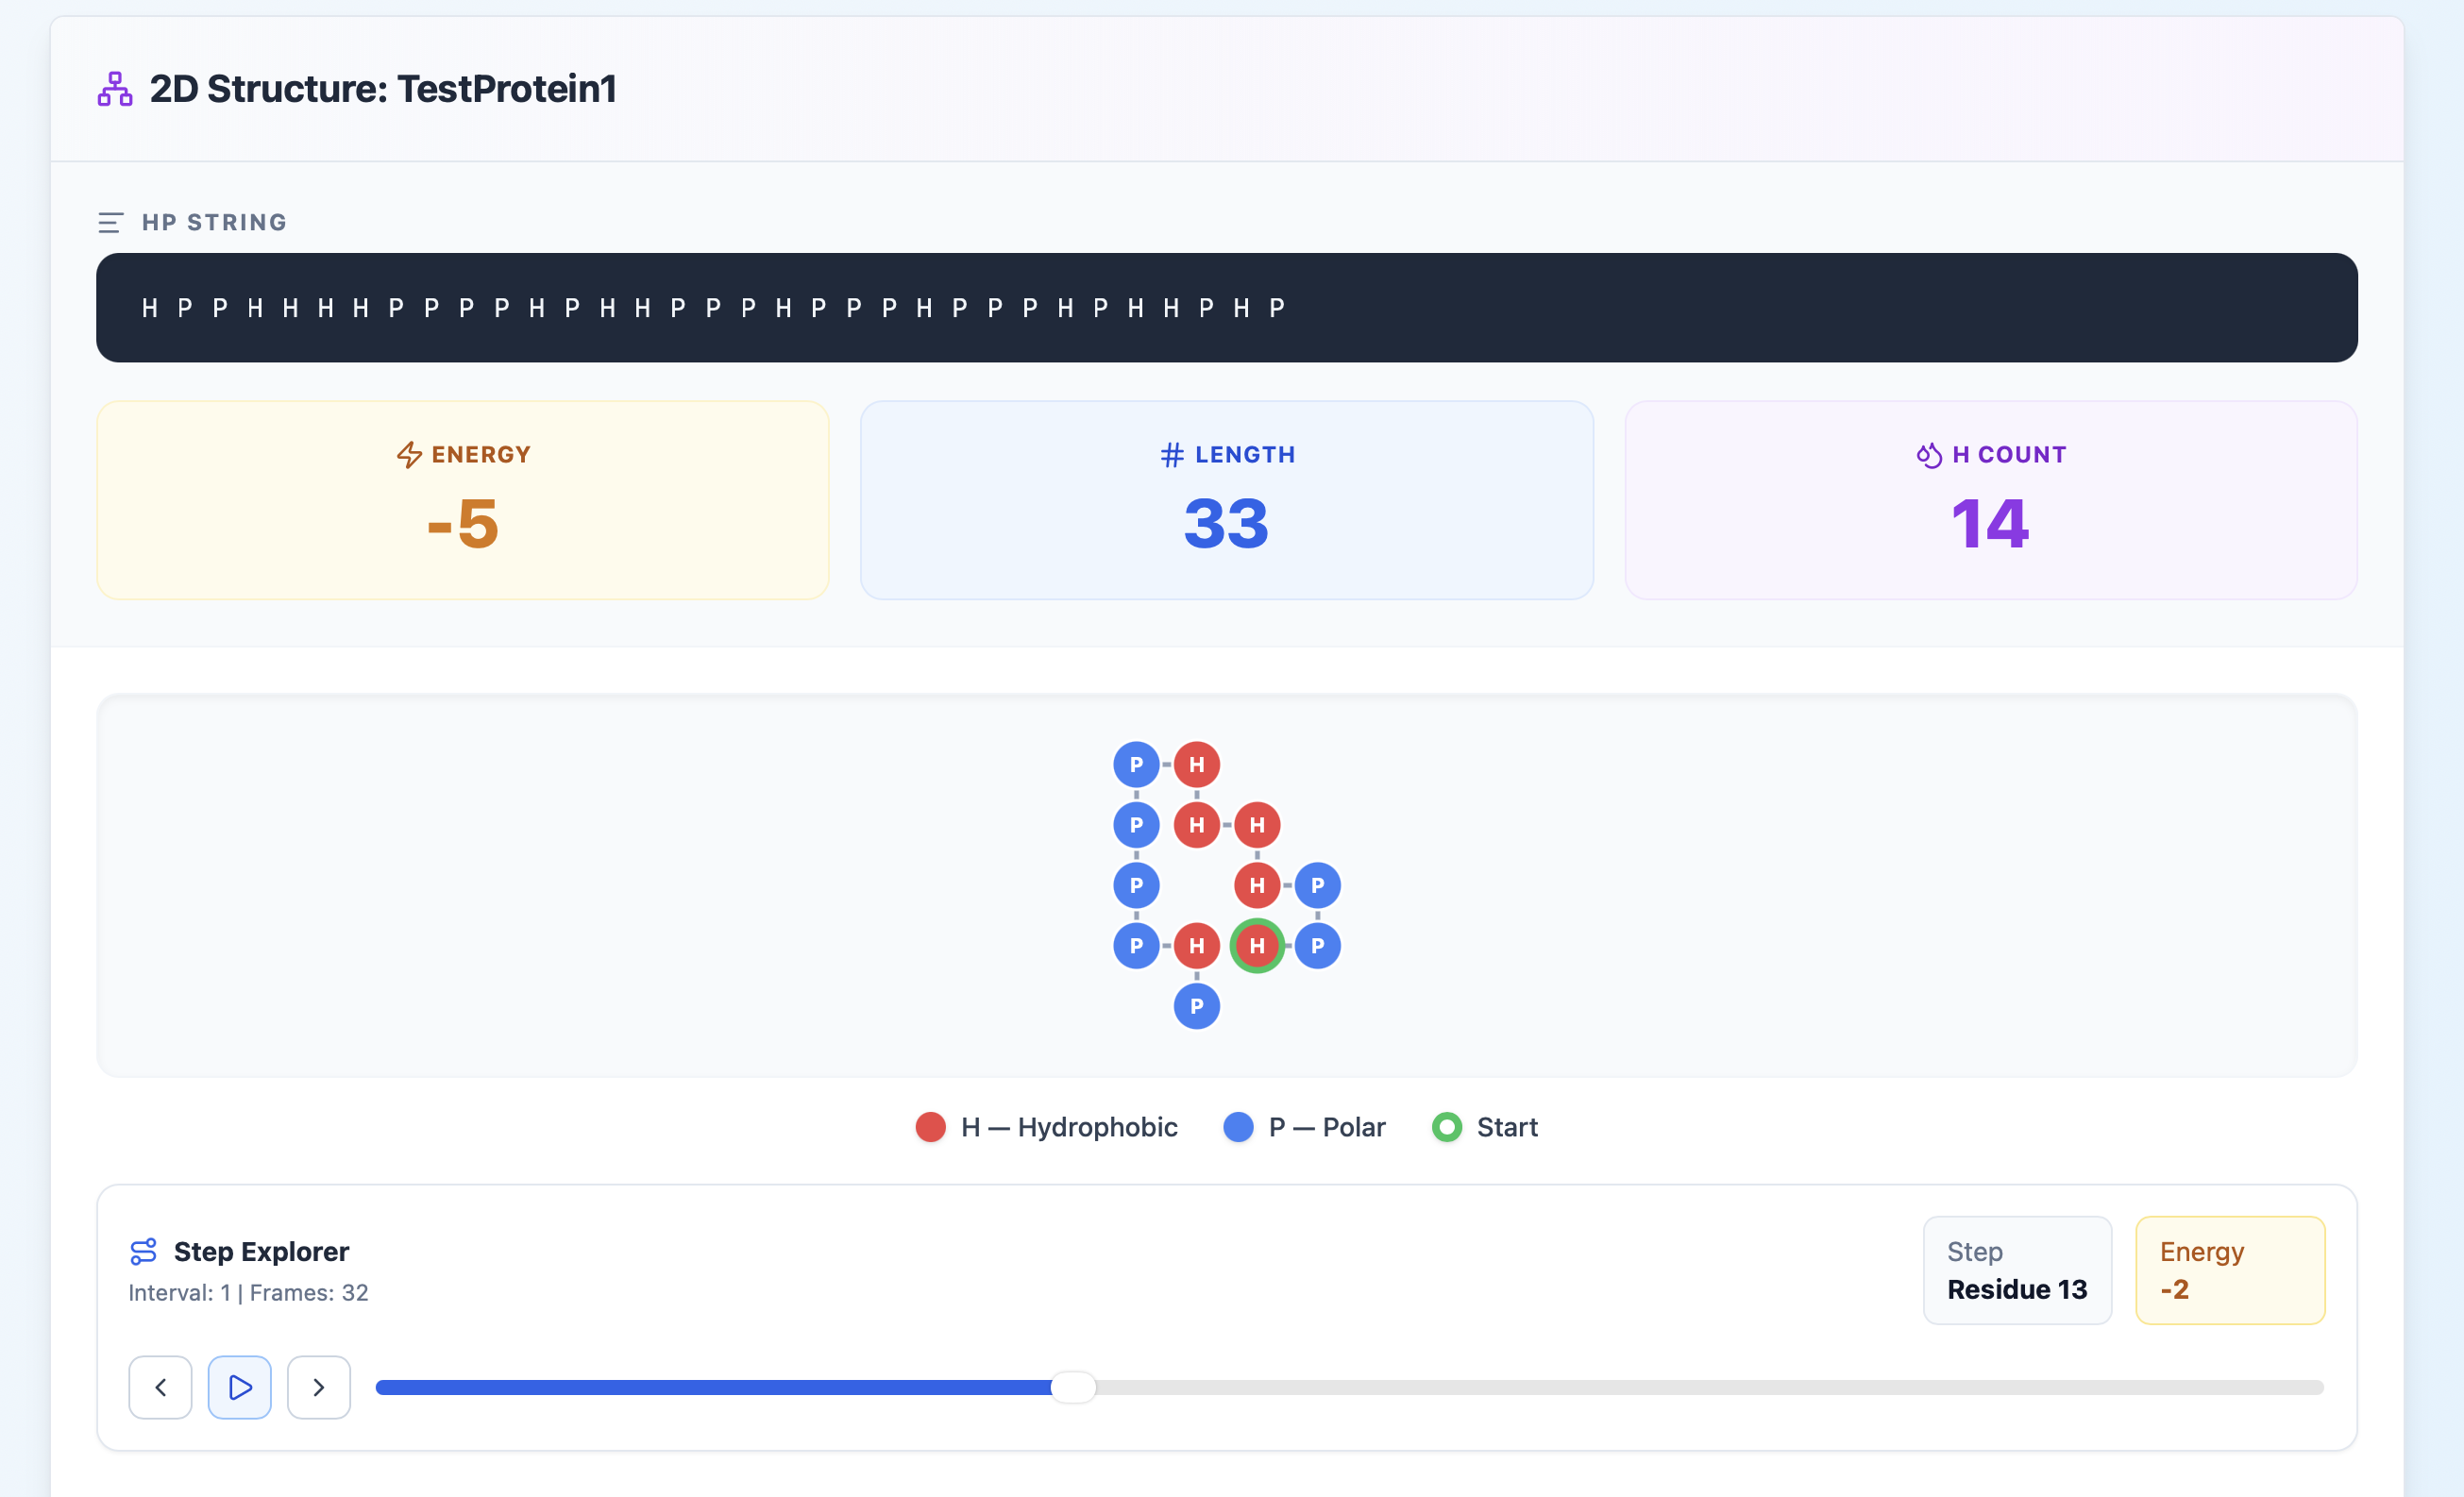
\includegraphics[width=\textwidth,height=0.70\textheight,keepaspectratio]{Figuras/2dStructure3.png}
\caption[2D HP step explorer: intermediate folding frame]{Intermediate folding frame in the 2D HP step explorer. The visualization makes it possible to inspect how local turns and hydrophobic contacts emerge before the final conformation is reached.}
\label{fig:appendix_2d_structure_step_intermediate}
\end{figure}
\FloatBarrier

\begin{figure}[!htbp]
\centering
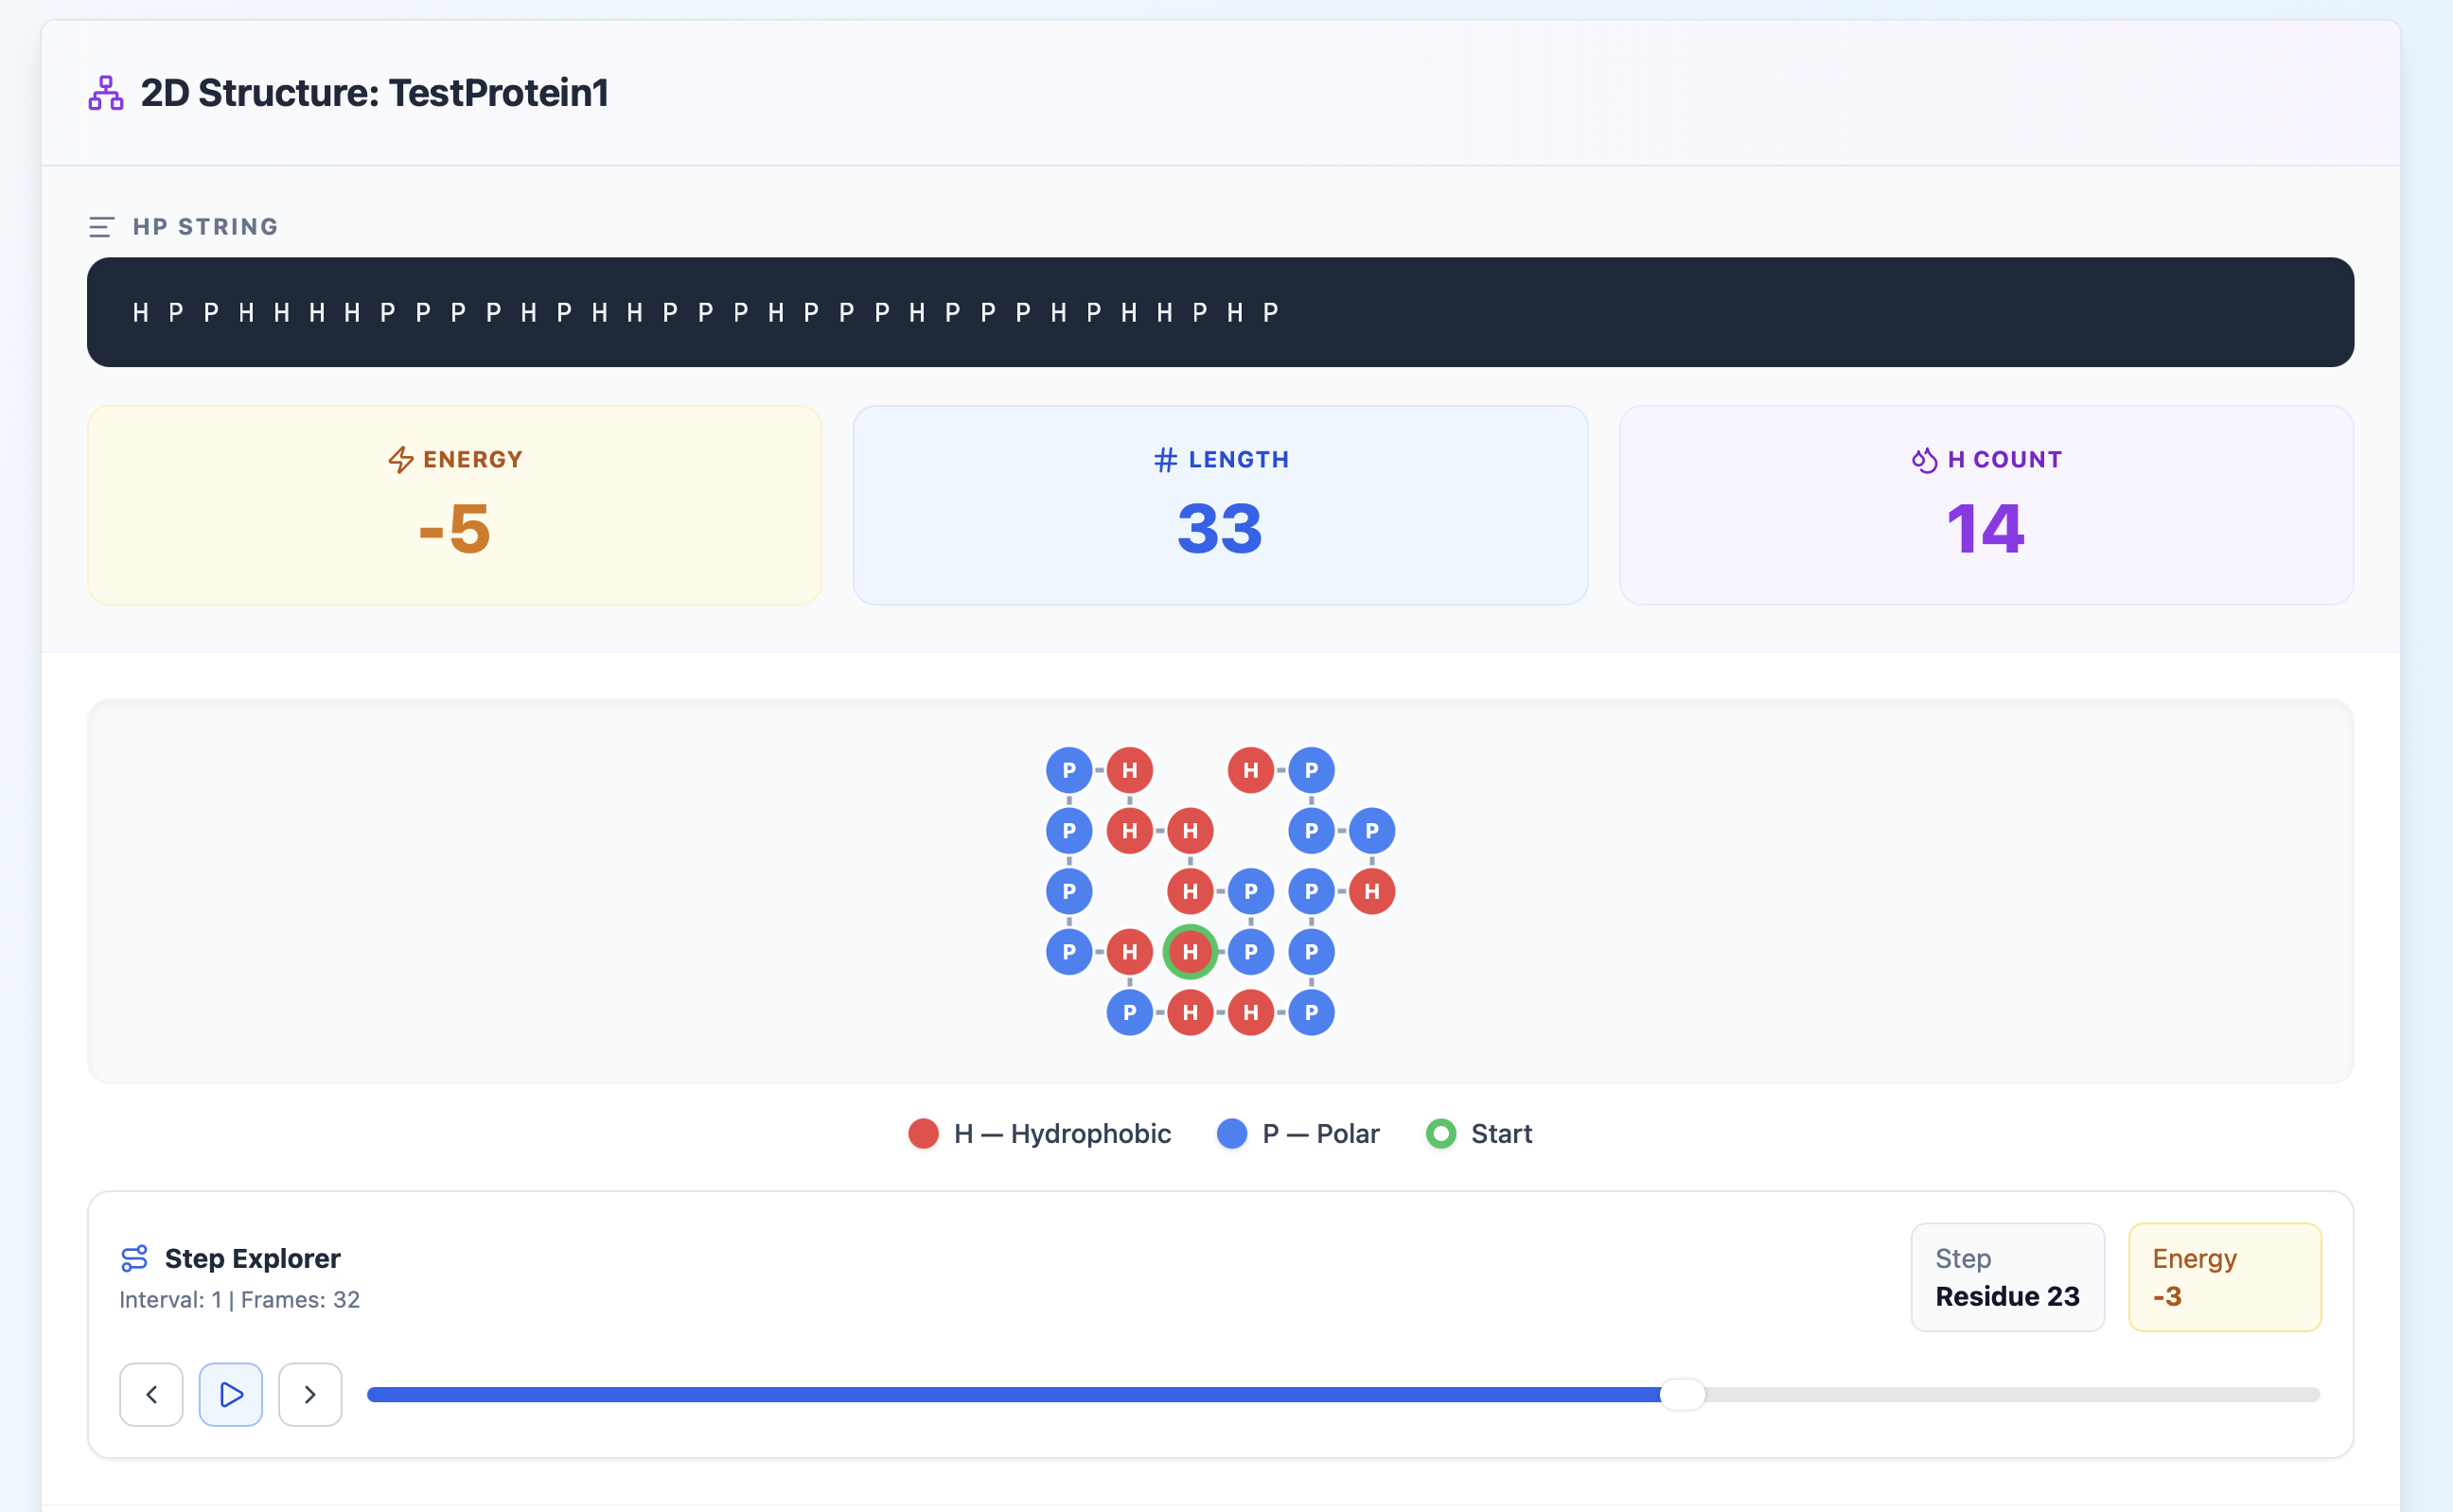
\includegraphics[width=\textwidth,height=0.70\textheight,keepaspectratio]{Figuras/2dStructure4.png}
\caption[2D HP step explorer: late folding frame]{Late folding frame in the 2D HP step explorer. The slider position and step counter allow the user to compare this near-final state with earlier conformations.}
\label{fig:appendix_2d_structure_step_late}
\end{figure}
\FloatBarrier

\begin{figure}[!htbp]
\centering
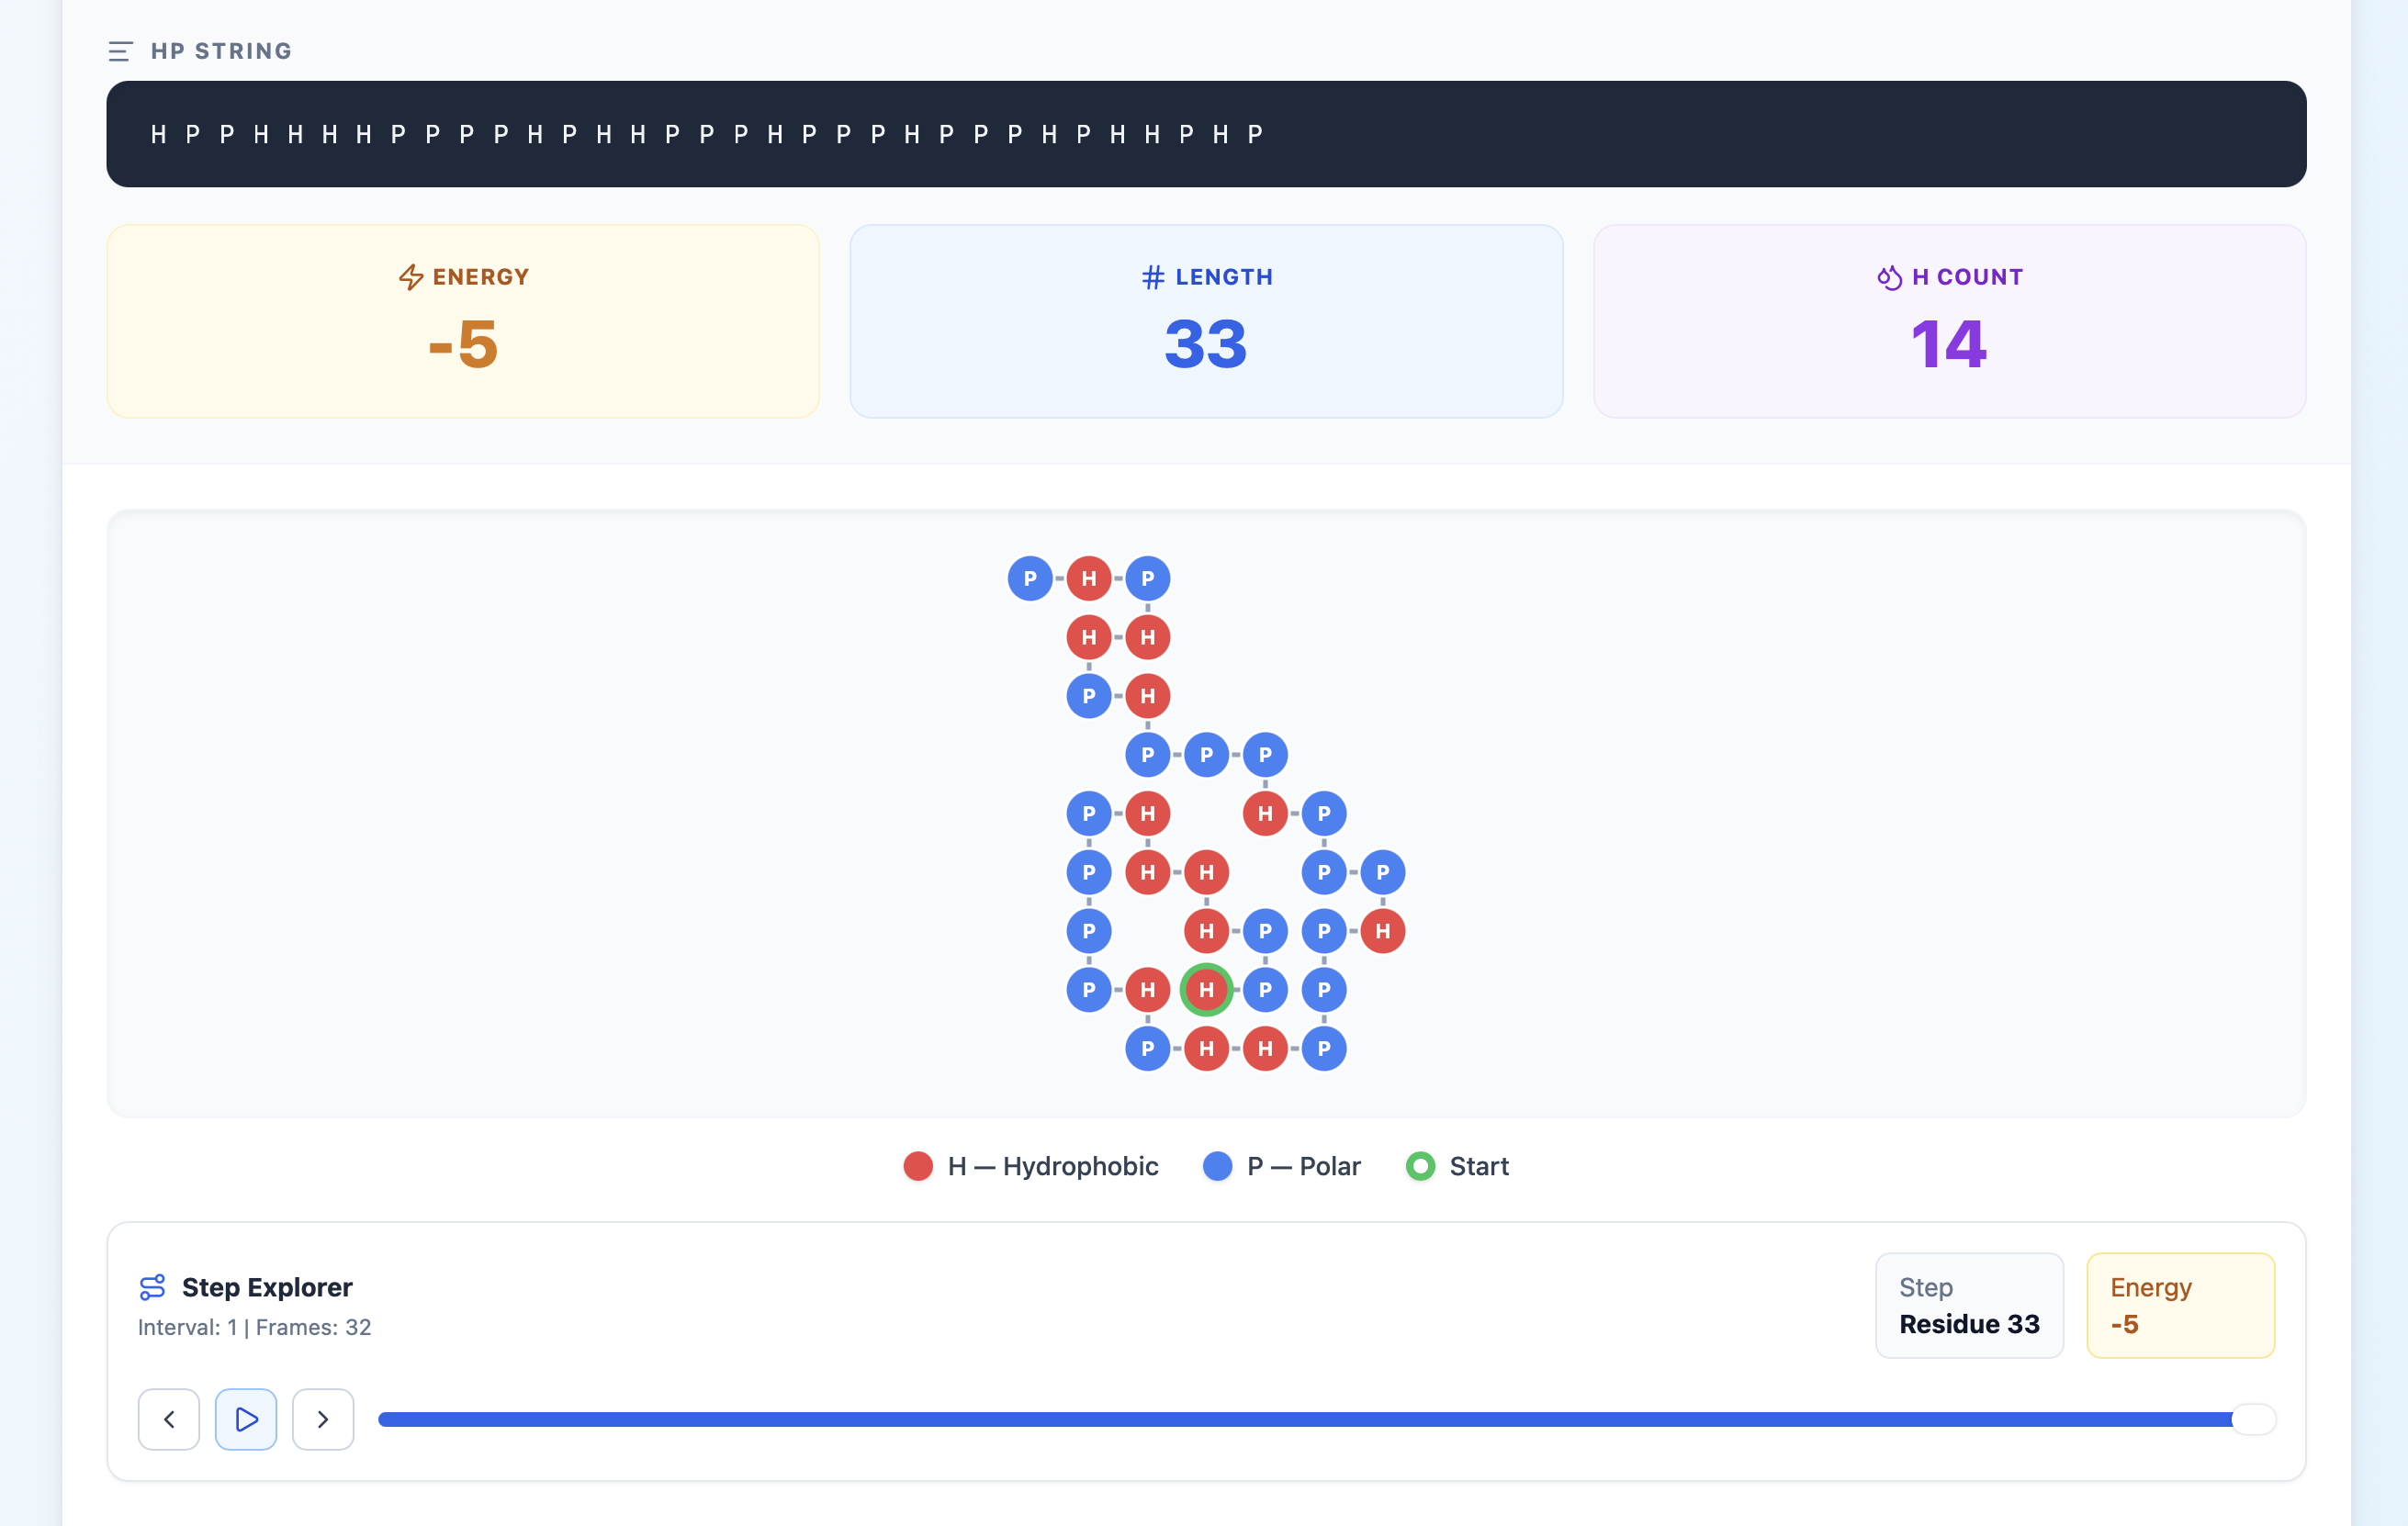
\includegraphics[width=\textwidth,height=0.70\textheight,keepaspectratio]{Figuras/2dStructure5.png}
\caption[2D HP step explorer: final frame]{Final 2D HP structure generated by the platform. The completed lattice conformation is shown together with the HP string, final energy, sequence length, hydrophobic residue count, and final step-explorer position.}
\label{fig:appendix_2d_structure_step_final}
\end{figure}
\FloatBarrier

\begin{figure}[!htbp]
\centering
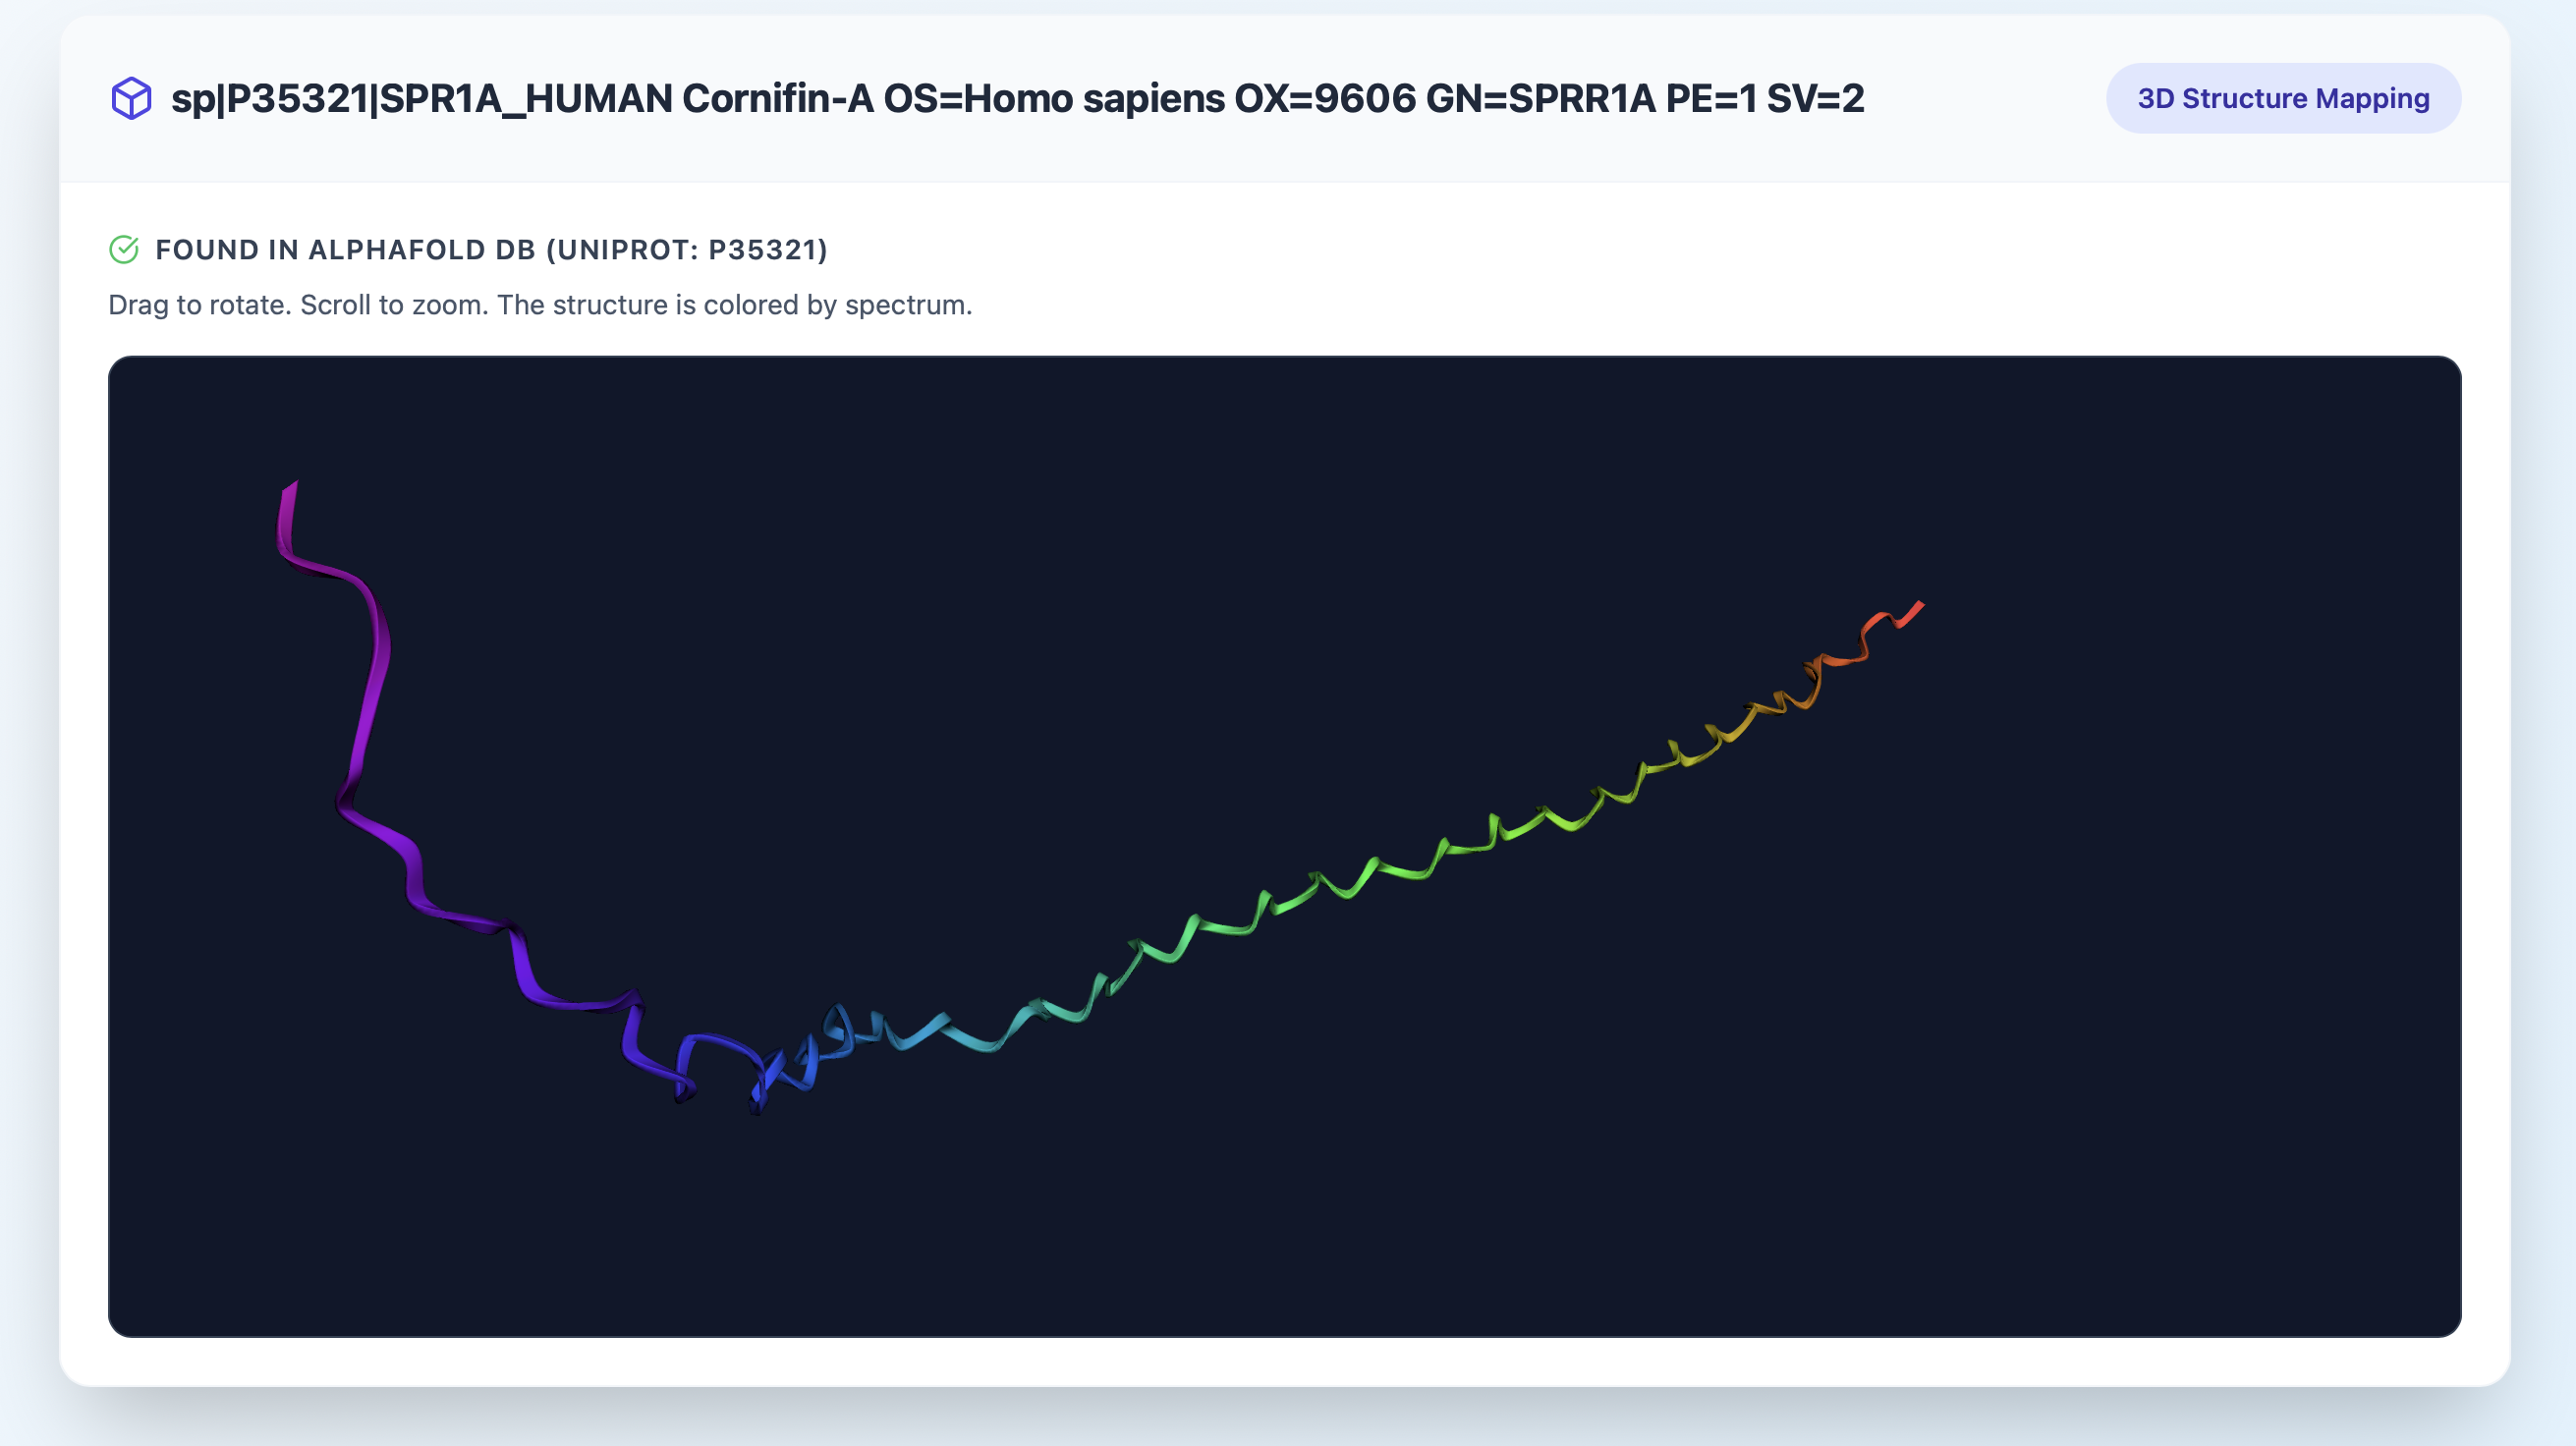
\includegraphics[width=\textwidth,height=0.76\textheight,keepaspectratio]{Figuras/3dStructureView.png}
\caption[3D structure visualization screen]{3D structure visualization screen. The platform retrieves known structures from AlphaFold DB or falls back to ESMFold for sequence-based prediction when necessary.}
\label{fig:appendix_3d_structure}
\end{figure}
\FloatBarrier
% !TEX root = ../main.tex
